\chapter{Diagramme de Gantt}

Le diagramme de Gantt, montré à la figure \ref{fig:Gantt} est un outil qui permet de visulaliser l'ensemble du projet au fil du temps. On y retrouve les tâches essentielles au bon fonctionnement du projet ainsi que les plages de teemps prévues pour chacunes. Les tâches sont également reliées entre elles, puisque certaines parties du projet ne peuvent être accompliques que si d'autres sont terminées. Par exemple, il faut d'abord avoir construit la station de recharge pour pouvoir la détecter.

\begin{figure}[ht]
    \centering
    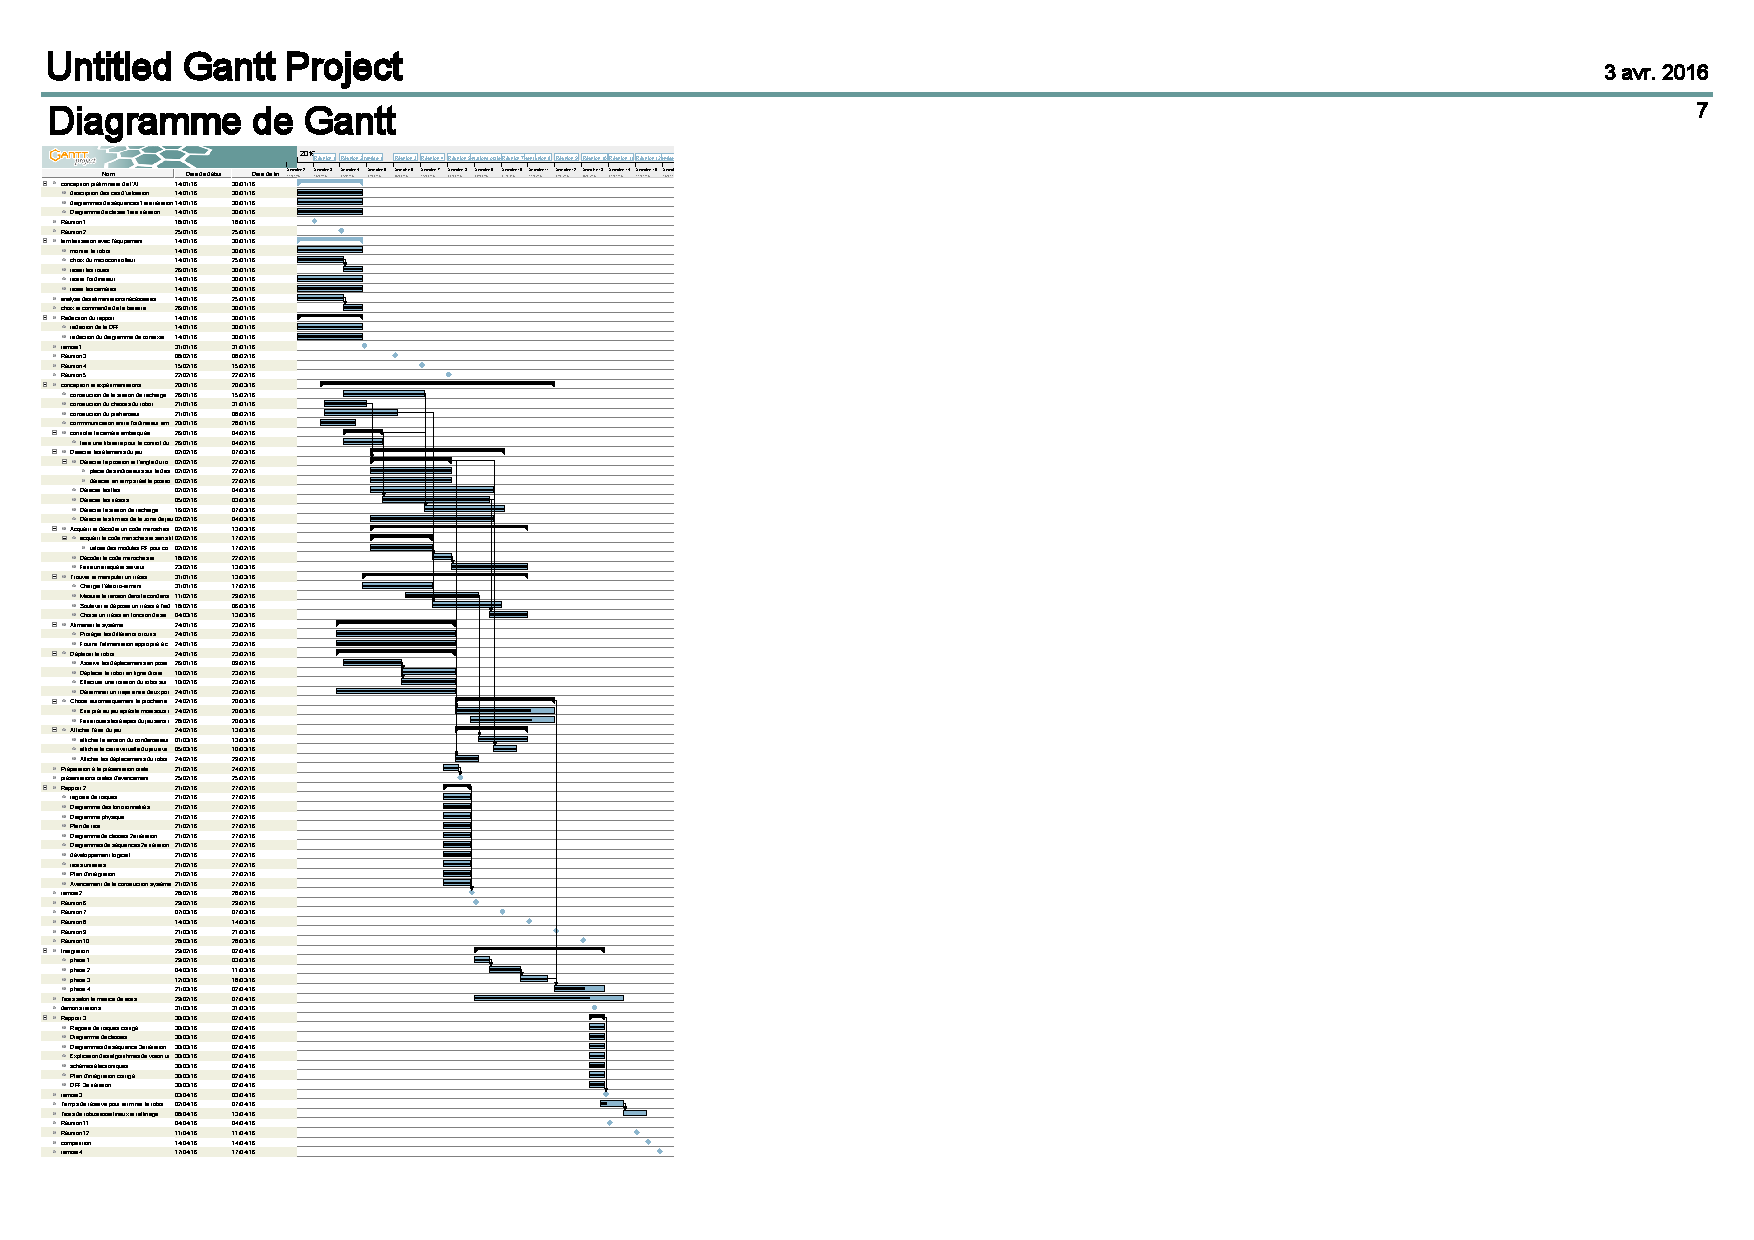
\includegraphics[scale=1, trim = 0 0 16cm 2.5cm, clip]{resources/gantt.pdf}
    \caption{Diagramme de Gantt}
    \label{fig:Gantt}
  \end{figure}